%%%%%%%%%%%%%%%%%%%%% ONLINE RELEASE %%%%%%%%%%%%%%%%%%%%

\chapter{Introduction}\label{chahpter:introduction}

Any complex surface can be recreated by blending or layering an arbitrary number of different less complex base materials.\footnote{The term \emph{material} can have a variety of different meanings within computer graphics and beyond, see section \ref{chapter:materials}.} Material layering is becoming an increasingly popular approach in recreating real world surface complexity for video games. Many \emph{AAA} games use this approach for their shading workflow (e.g., \cite{naugthy2016uncharted, witcher2015cdproject, order2015readyatdawns, paragon2016epic, gears2016coalition}). 

The growing importance of material layering is accompanied by three big trends within the video game industry. Content creation seems to shift more and more into the game engines. \emph{The Coalition}, \emph{Ready at Dawn} and \emph{Epic Games} transfer a big part of the material pipeline into the engine \cite{colin2017GearsOfWar, moore2017pipeline, neubelt2013crafting}. \emph{Unreal Engine 4 (UE4)} and \emph{Unity} provide many built in art tools (e.g., the shader graphs). Different 3rd party tools use live links to visualize changes directly within the game engine (e.g., \emph{Motion Builder} and \emph{Substance Painter}). Tools like \emph{Houdini} and \emph{Substance Designer} use plug-ins to enable working from within the engine. Further, a physical plausible workflow is preferred over a visual one. This improves consistency of assets across different lighting setups. It also increases consistency across different artists. Nowadays most 3D applications support a physically based rendering (PBR) shading workflow. Asset creation shifts more and more towards procedural techniques \cite{price2018ai}. 

There are many different approaches to layer and blend materials. Each one has its own advantages and disadvantages. The different methods will be explained later in this work. A major investigation focus for the analysis of the material layering methods for interactive, virtual environments\footnote{In this work an interactive, virtual environment is an artificial world provided by a computer. Its goal is to provide for an completely immersive world that is different from the players physical location \cite[p.\,9,\,30]{jerald2015vr}\cite[p.\,743]{gregory2015game}.} is about balancing visual appearance, technical constraints and limited production resources. Decomposing a complex surface into smaller, manageable elements is good way to split a task into smaller, less complex parts. Figure \ref{fig:dynamicMaterialBlending} shows an example of how a complex material can be recreated by combining a set of more generic materials. Splitting up a surface into smaller components can be beneficial from an artistic, production and technical point of view. Subproblems can be handled individually.     
 

 
\begin{figure}
	\centering
	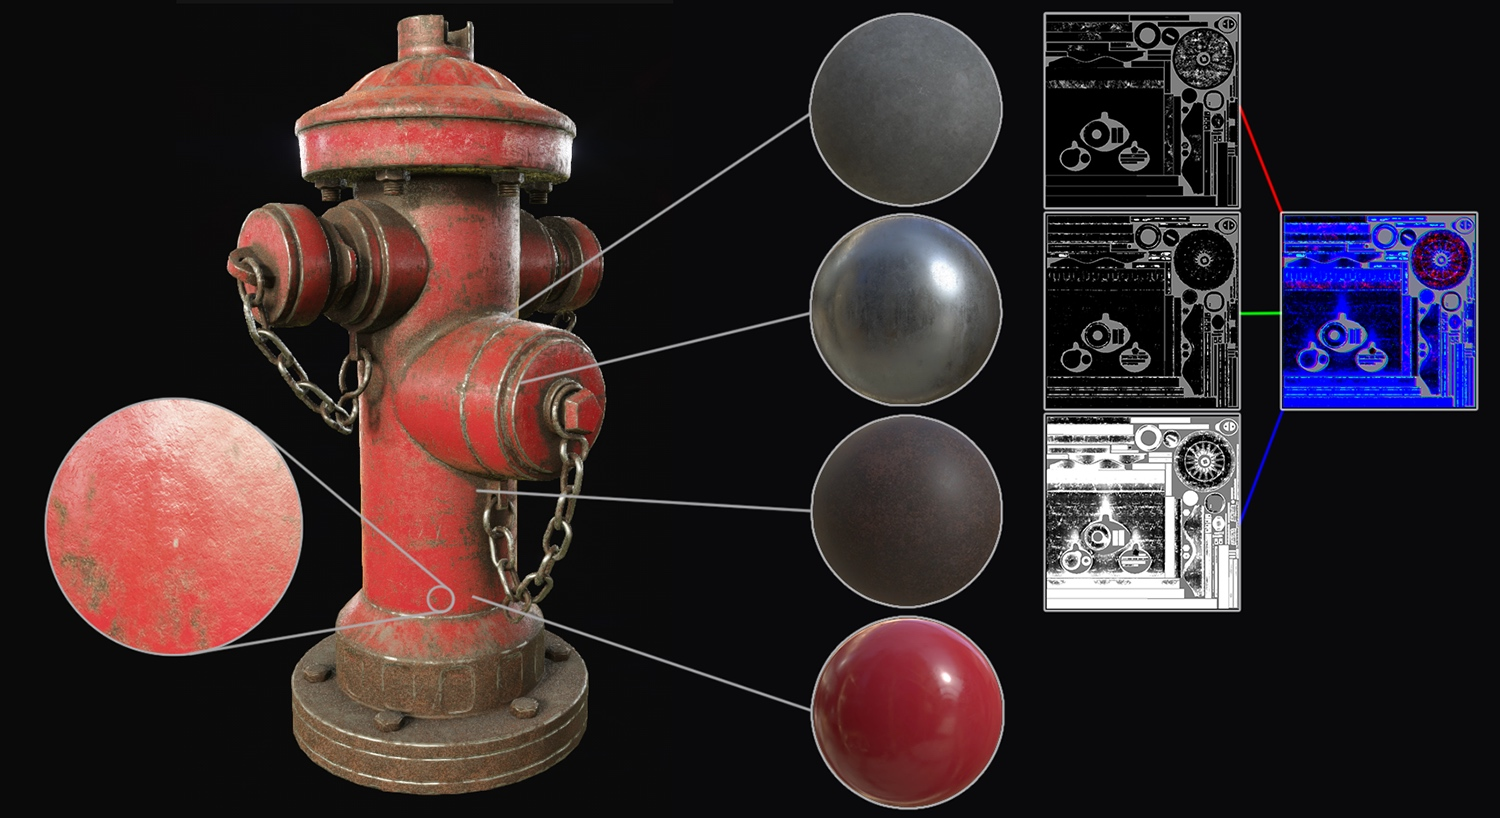
\includegraphics[width=0.7\linewidth]{images/01cha_01_dynamicMatBlend.jpg}
	\caption{Shading with pattern layering. This image illustrates the basic concept of the pattern layering. Pattern layering represents the most relevant material layering method for real-time applications. The fire hydrant is composed of 4 different tillable base materials. These base materials (dirt, clean metal) are blended by using the masks on the right. Image source: \cite{noguer2016layerHydrant}.}
	\label{fig:dynamicMaterialBlending}
\end{figure}



With this work, I will provide a proposal for material layering related design patterns, to support the decision making process while creating layered materials. To further elaborate why material layering is an important technique for creating large scale virtual environments, I will give a brief example. Looking at the ruins of an old castle, you might see that there is a lot of complexity going on over a huge amount of space. There are probably different layers of stones, plaster, color and moss and all these layers blend together and show the history of the object. A real world example can be seen in figure \ref{fig:heidelbergCastle}.

\begin{figure}
	\centering
	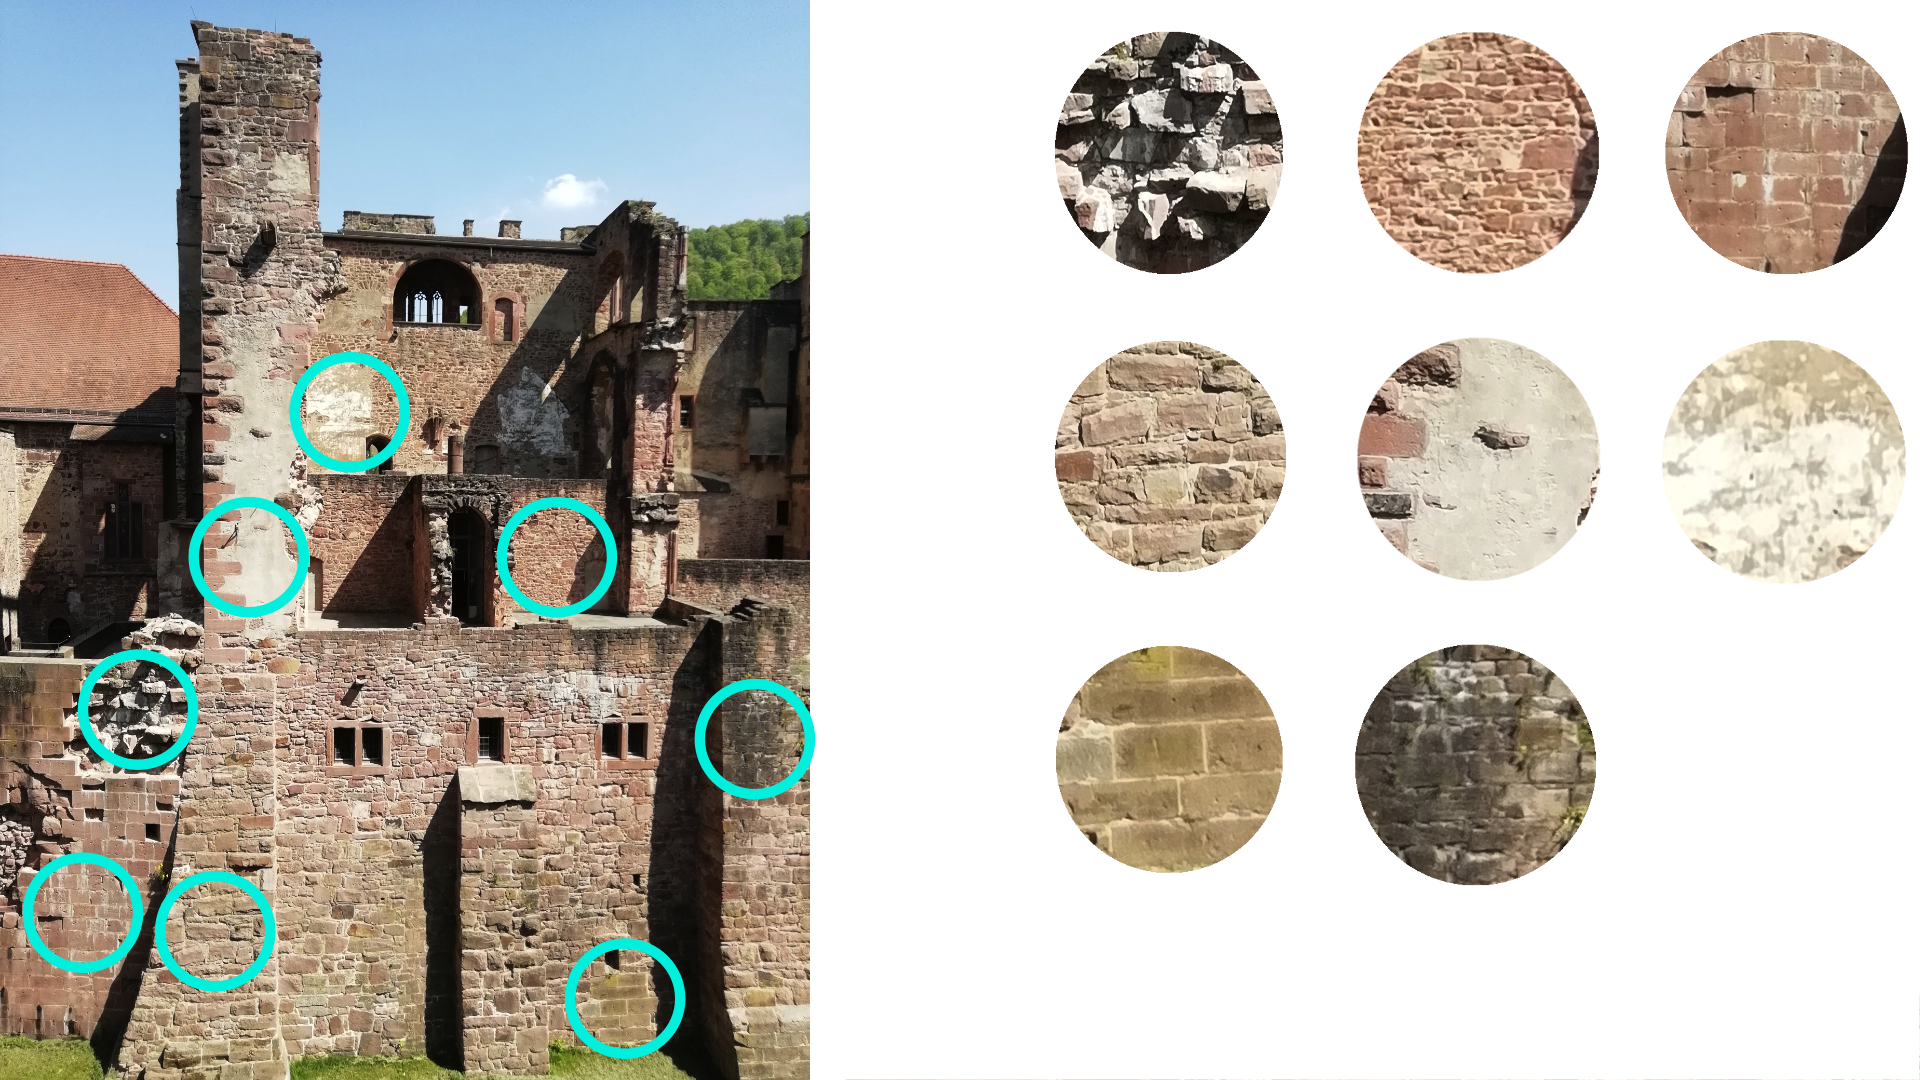
\includegraphics[width=0.8\linewidth]{images/01cha_02_HeidelbergCastle_mats.png}
	\caption{A challenging surface to recreate virtually. Recreating walls like this from the \emph{Heidelberg Castle} are a challenging task for 3D interactive environments. The main challenge is the rich amount of detail and surface variation across such a huge area of space. Recreating this richness of the surface with the stones in varying sizes, plaster, color and dirt is challenging from an artistic as well as a technical point of view. This becomes even more challenging as the player can move freely and seamlessly around, seeing the castle walls from near and far. One solution is to split the surface into different more generic base materials.}
	\label{fig:heidelbergCastle}
\end{figure}


\begin{figure}	
	\centering\small 
	\begin{tabular}{cc}
		\multicolumn{2}{c}{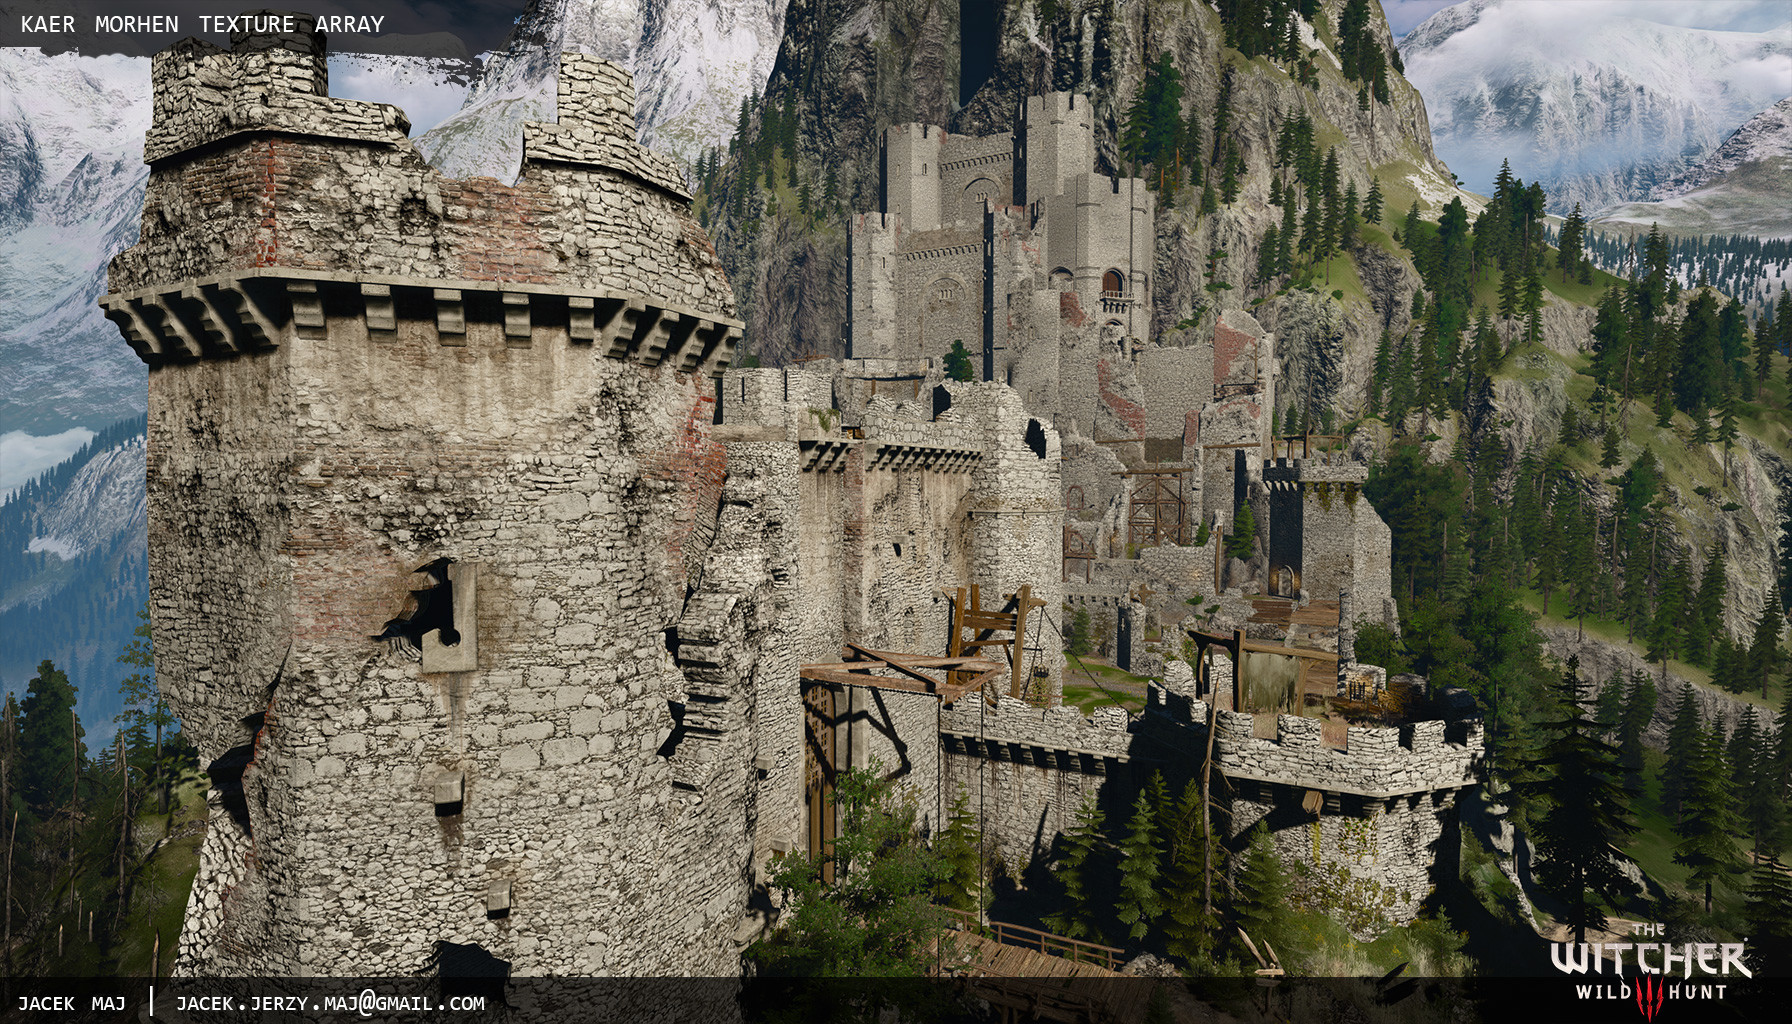
\includegraphics[width=0.8\textwidth]{images/01cha_03_jacek-maj-km-walls-04.jpg}} \\
		%	~~\raisebox{25mm}{(a)}} \\
		\multicolumn{2}{c}{(a)} \\
		[6pt]	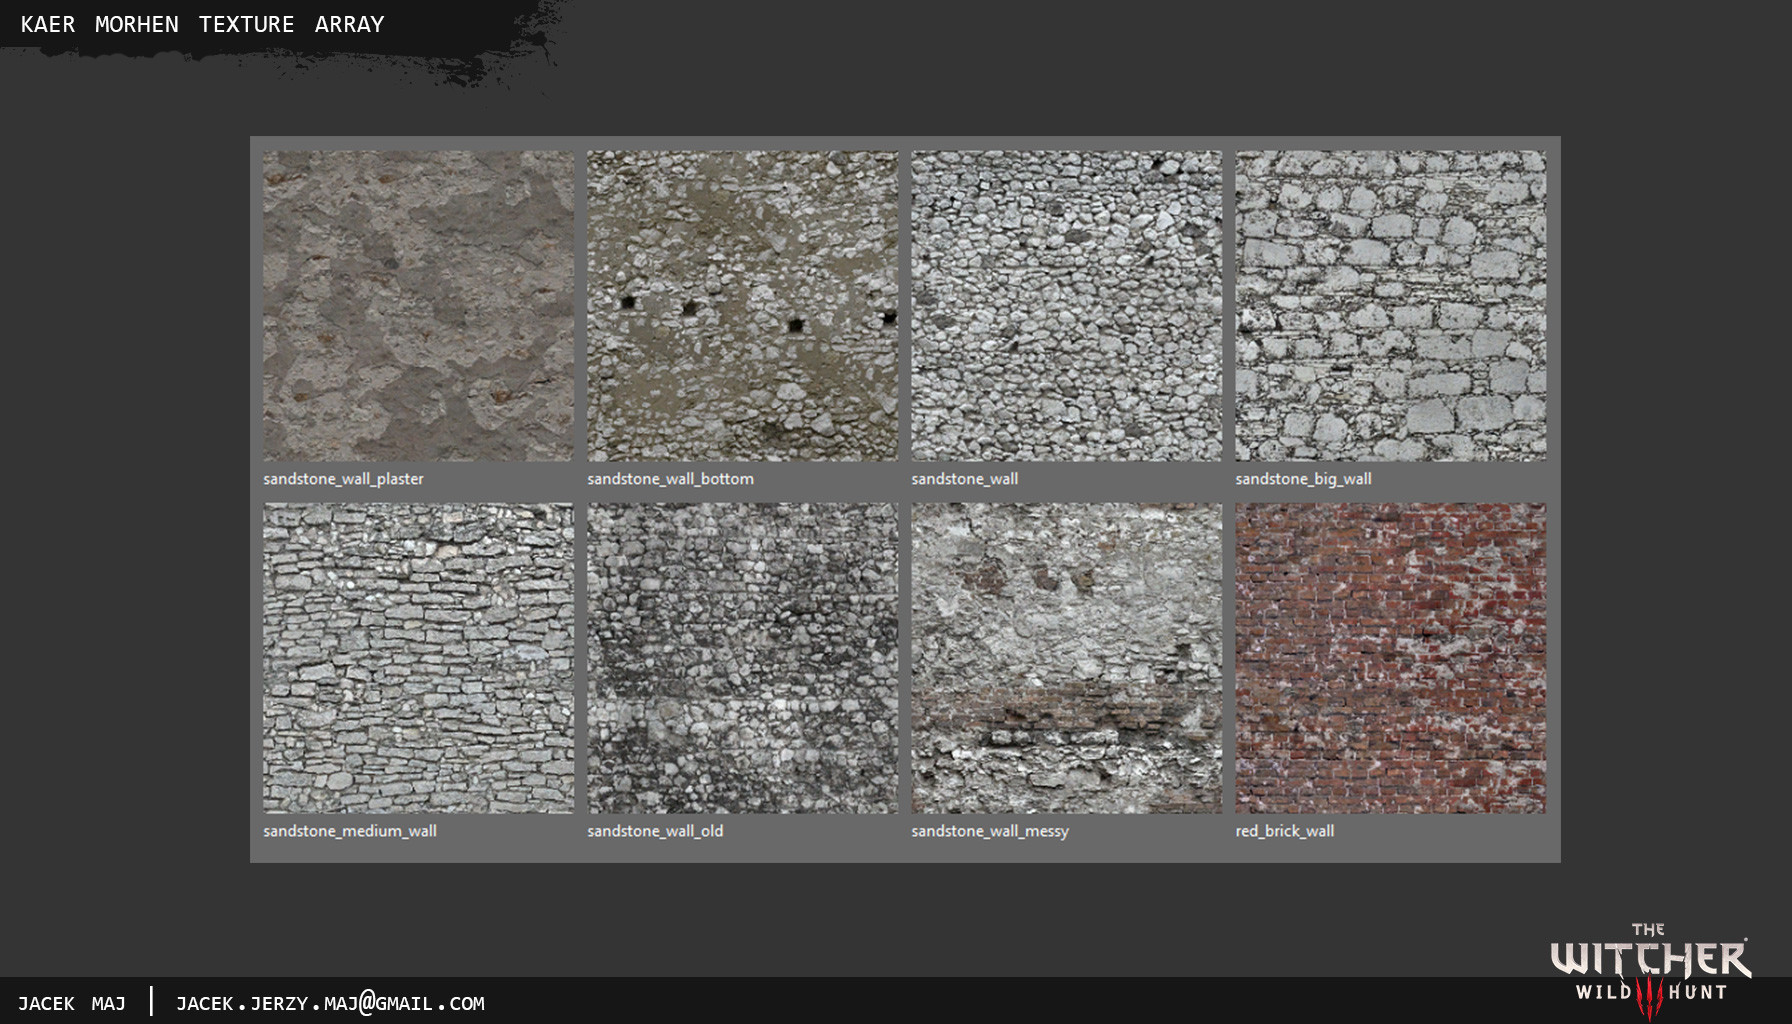
\includegraphics[width=0.4\textwidth]{images/01cha_04_jacek-maj-km-textures.jpg} &
		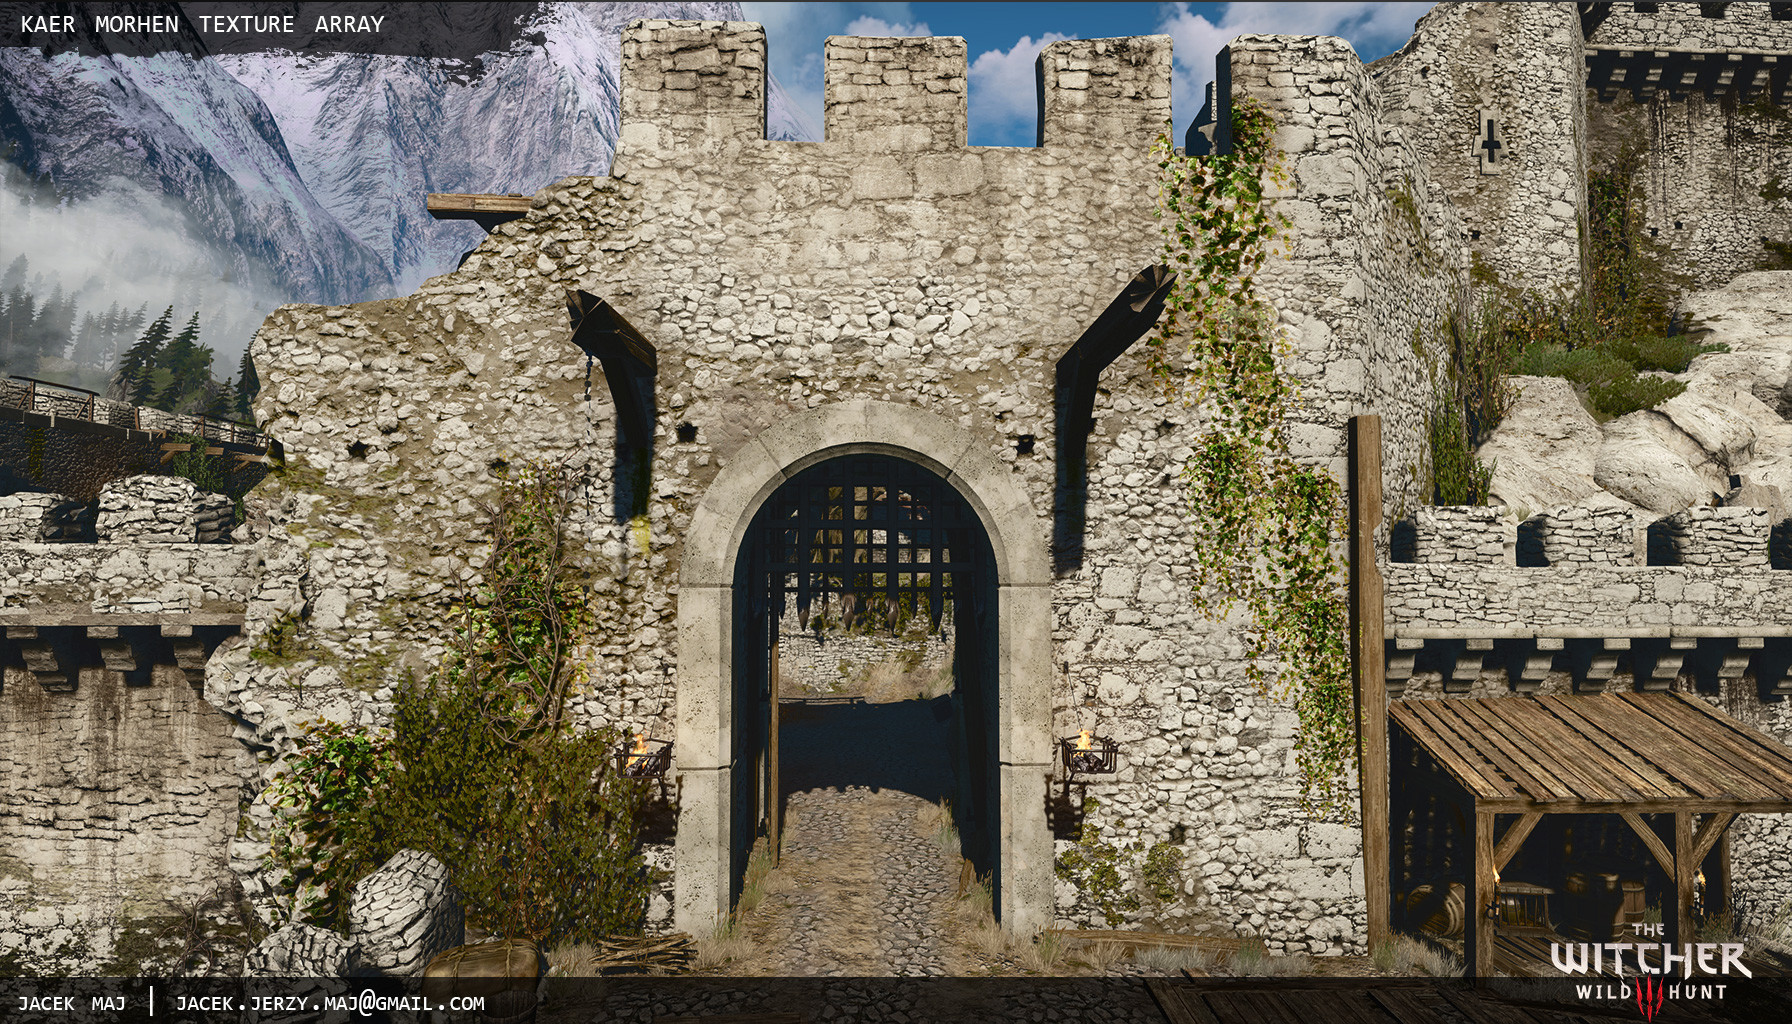
\includegraphics[width=0.4\textwidth]{images/01cha_05_jacek-maj-km-walls-01.jpg}
		\\
		(b) & (c)
		\\[6pt]	
	\end{tabular}
	\caption{Multitexture materials used for the buildings in \emph{Witcher 3} \cite{witcher2015cdproject}. Figure (a) shows the castle \emph{Kaer Morhen}. The walls of the castle are textured by layering different smaller scale textures, shown in figure (b). In combination with different masks, layering and parametric methods, it is possible to ensure a high texel density even from a closer view (c). Image source: \cite{maj2016witcherMaterial}. }
	\label{fig:witcherArchitectualMaterial}
\end{figure}


The wall surface\footnote{The term surface is further specified in section \ref{sec:surface}.} indicates the age, usage, interaction: Was it exposed to nature? Was it taken care of or simply left to decay? Capturing this kind of object history is more than just creating an interesting visual. It plays a major role in creating a deep, interesting and appealing world. Decomposing the material into different independent base materials and analyze how each material is blended with the others makes the challenge much more manageable than trying to solve every problem at once. A side effect of creating solutions to smaller, less specific problems is the possibility to reuse and modify the components and share them. This is normally not possible for all-in-one solutions as every subpart is heavily interlinked. 

The visual appearance is only one part, a completely different thing is to make the game run smoothly in real-time. The available resources---e.g., memory, bandwidth, CPU, GPU etc.---are limited and have to be used efficiently to make this possible. Depending on projects, requirements and hardware, different components will create a bottleneck in the rendering pipeline. Staying with the example of a big castle wall, the first approach might be to texture the huge surface by covering it entirely with huge unique textures. This approach relies on giant texture files and is therefore risky to create a bottleneck either by extending the available memory or bandwidth. Another approach is to recreate the micro detail of the wall with actual 3D geometry. This method might work for a few objects but soon result in an enormous polycount and create a bottleneck in another part of the rendering pipeline. A probably better suited solution might be to use material layering. One way to do material layering is to use several tillable textures, blend and manipulate them with different methods and create a complex, large scale surface. \emph{The Witcher 3: Wild Hunt} \cite{witcher2015cdproject} used a similar approach to create wall materials as shown in figure \ref{fig:witcherArchitectualMaterial}. 

\section{Research Objective}

The goal of this thesis is to collect answers for recurring decisions regarding material layering in real-time applications. This thesis will cover bigger concepts behind common texture layering problems and is not intended as a step-by-step guide in how to implement a certain design. It will provide users with a tool set of tested methods to improve decision making concerning pattern based material layering. The different approaches to material layering are discussed in section \ref{cha:materialLayering}. In the end, the design patters should support game makers in populating a scene with a huge amount of appealing, distinctive and complex objects without extending the technical limitations of a first person real-time application. To do so, this work attempts to define design patterns to answer recurring problems regarding pattern based material layering. As a template for the pattern design I adopt the scheme presented by Erich Gamma et al. \cite{gamma1995design} and Jenifer Tidwell \cite{tidwell2010designing}. According to this template, design patterns themselves should contain the most important information like application, benefit and risk \cite[p.\,3]{gamma1995design}. See chapter \ref{chapter:designPatterns} for further details on design patterns. \emph{Weta Digial} evaluates new technologies and tools according to three major aspect: ``performance vs. correctness vs. artistic freedom'' \cite{weidlich2011thinking}. These same free factors play an essential role for evaluating the design patterns defined in this work;  
% avoid spaces 
\begin{description}
	\item[Artistic Freedom:] To what extend does the technique enable artists to reach a visual goal? What are the aesthetic limitations and downsides of the used method that are to be expected? 
	\item[Performance:] What is the impact of the method on performance? Which bottlenecks might the method lead to (e.g., memory, bandwidth, CPU, GPU). Might this method solve a performance issue I already have?   
	\item[Correctness:] How versatile, flexible and robust is the used method? Does it support an interactive, shared workflow and can sub-parts be reused, combined and shared? 
\end{description}
% avoid spaces
All test cases are based on opaque, physically based,\footnote{The term physically based is used to describe  methods that try to imitate the real world behavior by following the laws of physics \cite[p.\,1]{pharr2016physically}. In general, you can distinguish between physically correct and physically plausible approaches. While the former tries to stay as close to reality as possible, the latter deliberately chooses art-directability and performance before physical accuracy \cite[p.\,12]{burley2012physically}\cite[p.\,2]{wes2018comprehensivevol2}.} dielectric and metallic materials, not including advanced shading concepts like translucency, transparency, subsurface scattering and volumetrics. To make the results comparable, all test share a similar aesthetic goal in creating a photorealistic\footnote{The appearance of a photo realistic object should be close or indistinguishable from photographs. As human perception is subjective, this may vary from person to person \cite[p.\,4]{pharr2016physically}\cite[p.\,99]{akenine2008real}.} and vivid environment. Most design patterns were tested and evaluated in the production of \emph{Letzte Worte} \cite{letzteWorte2019game}. Neither the creation process of textures, their blending in a texturing software with the result of a single, baked texture nor the technical implementation are going to be part of the thesis.

 

\section{Structure of this Thesis}

Chapter \ref{cha:definitions} starts by defining the key terminology for this work. Chapter \ref{cha:materialLayering} provides an overview of the current development and state of the art. It gives an overview of the different concepts for material layering. Further, it discusses which methods are already relevant for real-time applications and which might become interesting in the near future. The thesis continues  by defining an abstract description model for pattern layering in chapter \ref{cha:partsOfLayeredShader}. This will be especially relevant to understand the structure and categorization of the design patterns. Chapter \ref{cha:implementationParametricLayering} focuses on the implementation of the previously theoretically described models. Before digging into the core of this work, a short spin is made to discuss design patterns from other industries. Chapter \ref{chapter:designPatterns} explains how these concepts can be transposed to this work. Chapter \ref{cha:patterns} presents a detailed catalog of design patterns. They are structured hierarchically and categorized thematically. This helps to easily navigate to the problem relevant patterns. Finally, chapter \ref{cha:discussion} concludes by presenting the results, limitations and prospects for  future research. 
